\documentclass[11pt,a4paper]{report}
\usepackage[textwidth=37em,vmargin=30mm]{geometry}
\usepackage{calc,xunicode,amsmath,amssymb,paralist,enumitem,tabu,booktabs,datetime2,xeCJK,xeCJKfntef,listings}
\usepackage{tocloft,fancyhdr,tcolorbox,xcolor,graphicx,eso-pic,xltxtra,xelatexemoji}

\newcommand{\envyear}[0]{2024}
\newcommand{\envdatestr}[0]{2024-11-12}
\newcommand{\envfinaldir}[0]{webdb/2024/20241112/final}

\usepackage[hidelinks]{hyperref}
\hypersetup{
    colorlinks=false,
    pdfpagemode=FullScreen,
    pdftitle={Web Digest - \envdatestr}
}

\setlength{\cftbeforechapskip}{10pt}
\renewcommand{\cftchapfont}{\rmfamily\bfseries\large\raggedright}
\setlength{\cftbeforesecskip}{2pt}
\renewcommand{\cftsecfont}{\sffamily\small\raggedright}

\setdefaultleftmargin{2em}{2em}{1em}{1em}{1em}{1em}

\usepackage{xeCJK,xeCJKfntef}
\xeCJKsetup{PunctStyle=plain,RubberPunctSkip=false,CJKglue=\strut\hskip 0pt plus 0.1em minus 0.05em,CJKecglue=\strut\hskip 0.22em plus 0.2em}
\XeTeXlinebreaklocale "zh"
\XeTeXlinebreakskip = 0pt


\setmainfont{Brygada 1918}
\setromanfont{Brygada 1918}
\setsansfont{IBM Plex Sans}
\setmonofont{JetBrains Mono NL}
\setCJKmainfont{Noto Serif CJK SC}
\setCJKromanfont{Noto Serif CJK SC}
\setCJKsansfont{Noto Sans CJK SC}
\setCJKmonofont{Noto Sans CJK SC}

\setlength{\parindent}{0pt}
\setlength{\parskip}{8pt}
\linespread{1.15}

\lstset{
	basicstyle=\ttfamily\footnotesize,
	numbersep=5pt,
	backgroundcolor=\color{black!5},
	showspaces=false,
	showstringspaces=false,
	showtabs=false,
	tabsize=2,
	captionpos=b,
	breaklines=true,
	breakatwhitespace=true,
	breakautoindent=true,
	linewidth=\textwidth
}






\newcommand{\coverpic}[2]{
    % argv: itemurl, authorname
    Cover photo by #2~~(\href{#1}{#1})
}
\newcommand{\makeheader}[0]{
    \begin{titlepage}
        % \newgeometry{hmargin=15mm,tmargin=21mm,bmargin=12mm}
        \begin{center}
            
            \rmfamily\scshape
            \fontspec{BaskervilleF}
            \fontspec{Old Standard}
            \fontsize{59pt}{70pt}\selectfont
            WEB\hfill DIGEST
            
            \vfill
            % \vskip 30pt
            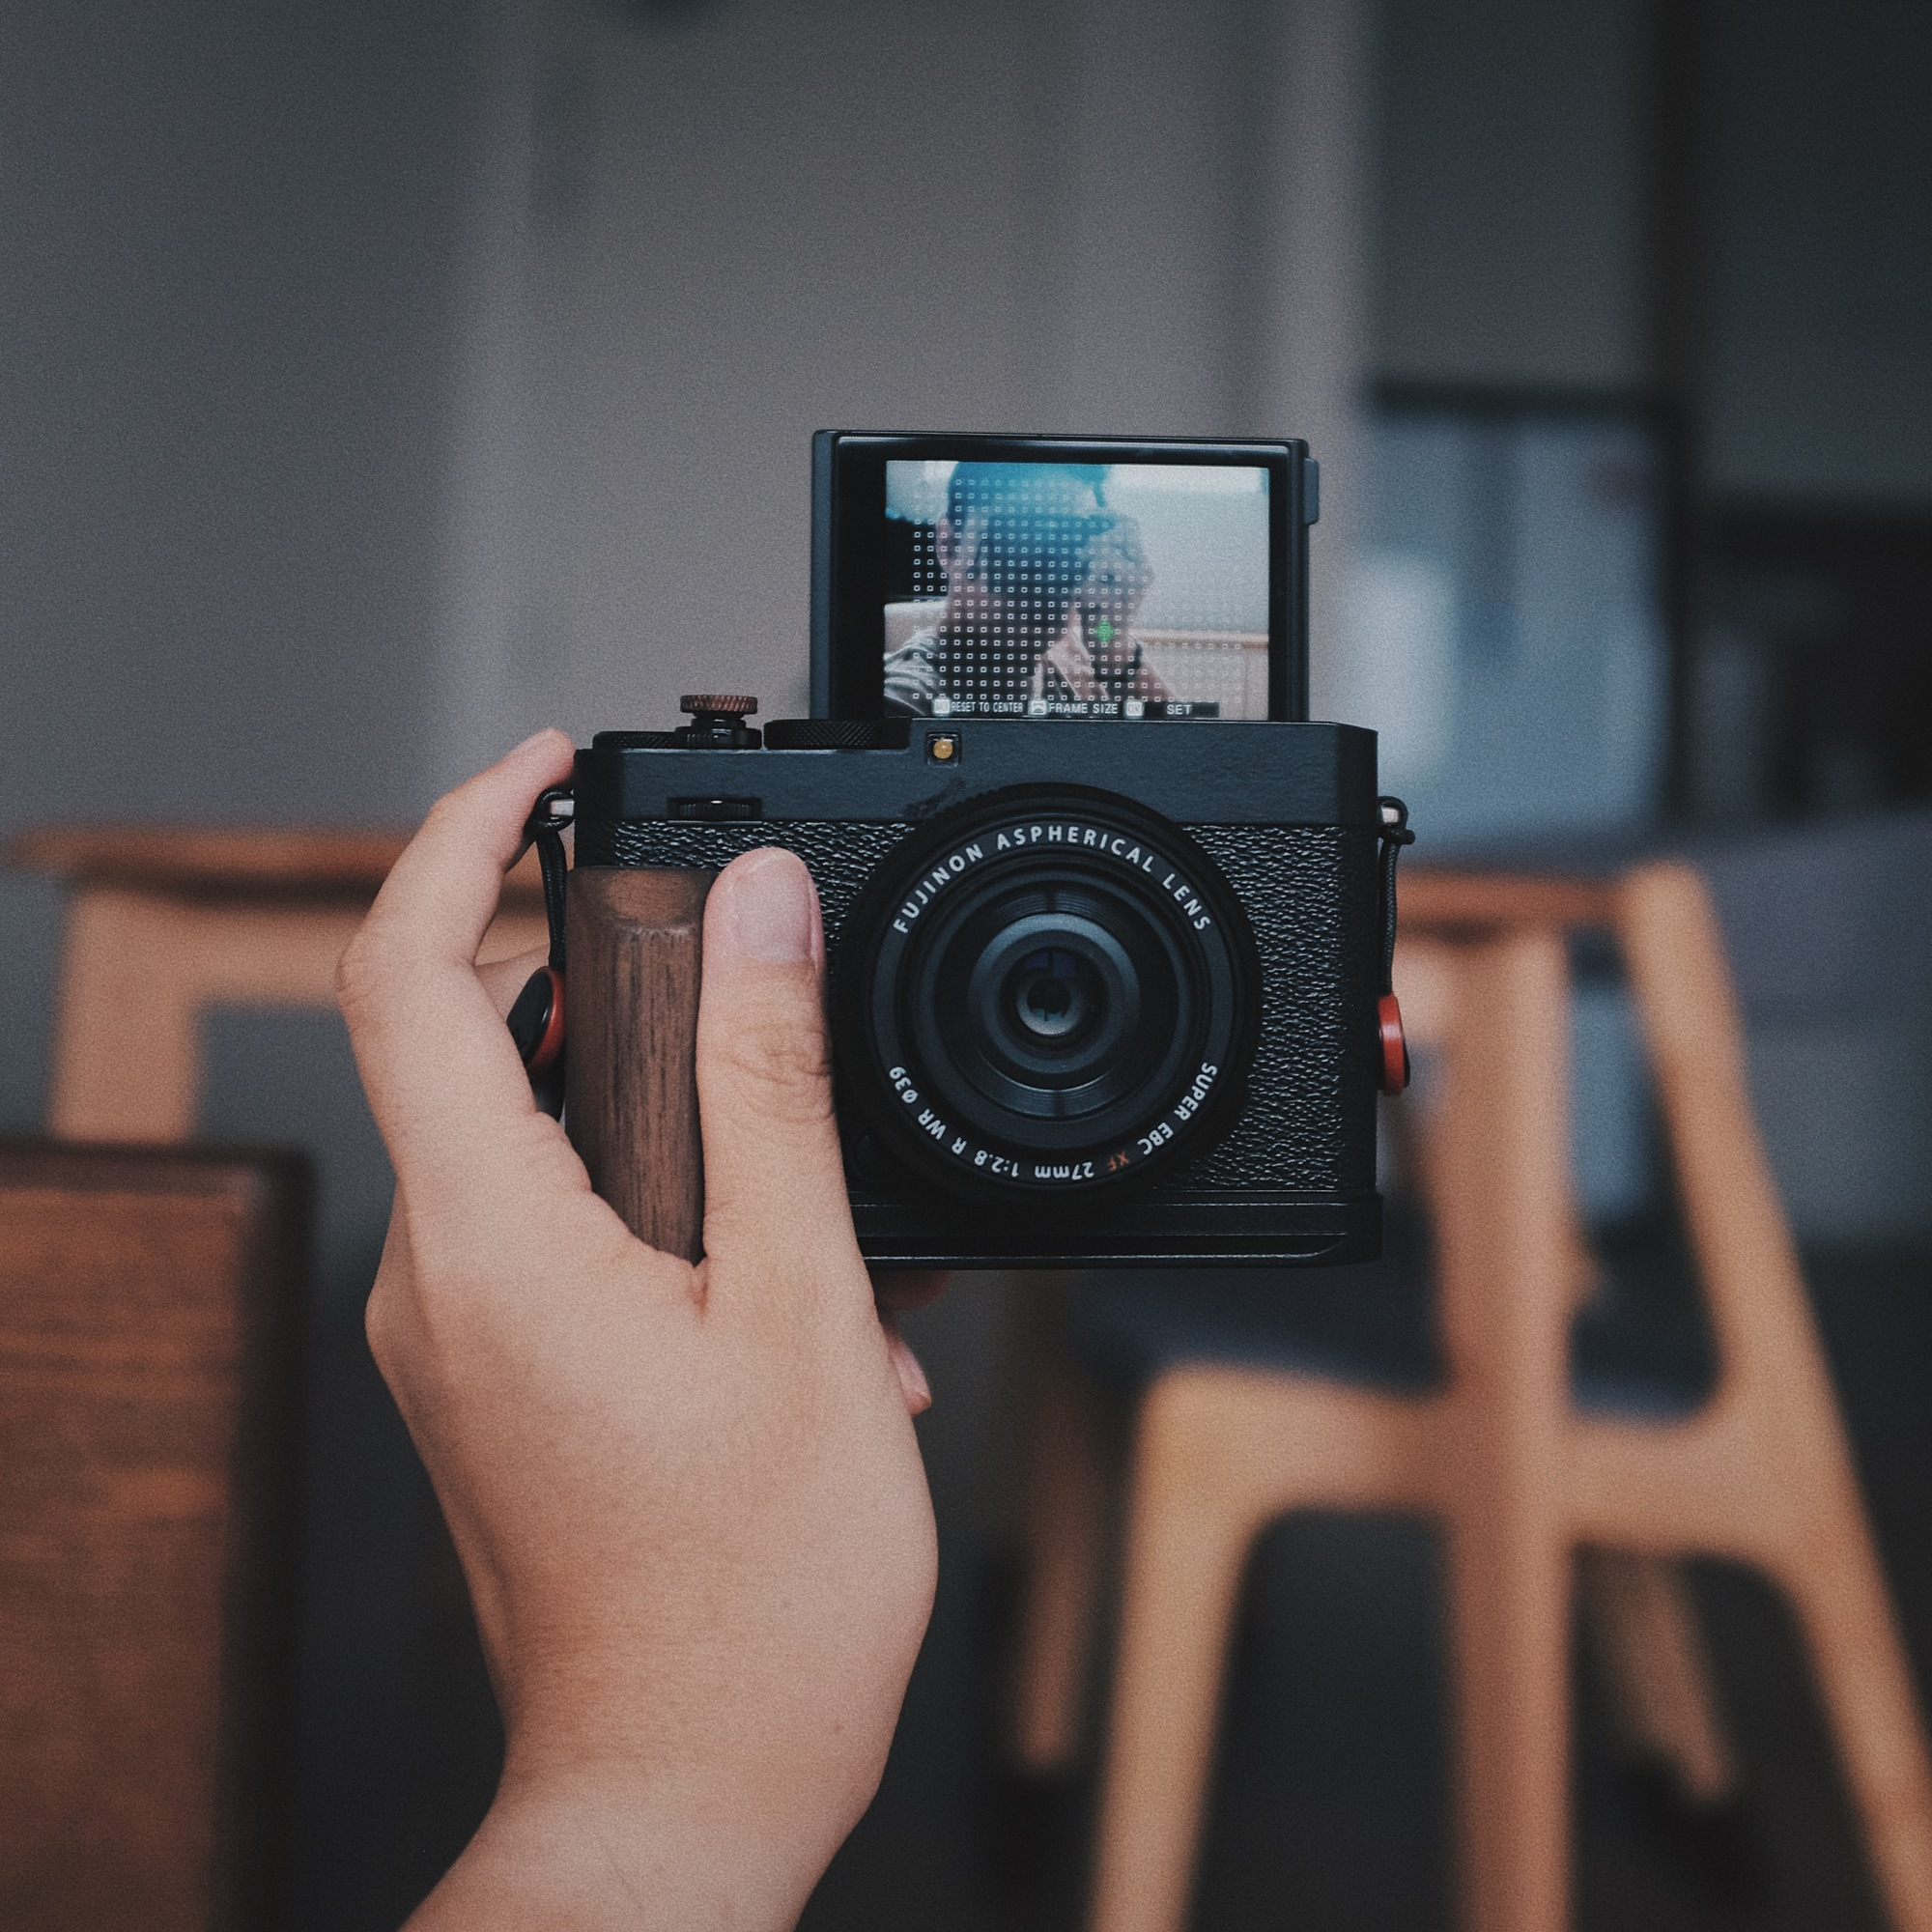
\includegraphics[width=\linewidth]{\envfinaldir/coverpic-prod.jpg}\par
            % \vskip 30pt
            \vfill

            \normalsize\rmfamily\scshape
            \copyright{} The Web Digest Project \hfill\large \envdatestr
        \end{center}
    \end{titlepage}
    % \restoregeometry
}
\newcommand{\simplehref}[1]{%
    \textcolor{blue!80!green}{\href{#1}{#1}}%
}
\renewcommand{\contentsname}{\center\Huge\sffamily\bfseries Contents\par\vskip 20pt}
\newcounter{ipartcounter}
\setcounter{ipartcounter}{0}
\newcommand{\ipart}[1]{
    % \vskip 20pt
    \clearpage
    \stepcounter{ipartcounter}
    \phantomsection
    \addcontentsline{toc}{chapter}{#1}
    % \begin{center}
    %     \Huge
    %     \sffamily\bfseries
    %     #1
    % \end{center}
    % \vskip 20pt plus 7pt
}
\newcounter{ichaptercounter}
\setcounter{ichaptercounter}{0}
\newcommand{\ichapter}[1]{
    % \vskip 20pt
    \clearpage
    \stepcounter{ichaptercounter}
    \phantomsection
    \addcontentsline{toc}{section}{\numberline{\arabic{ichaptercounter}}#1}
    \begin{center}
        \Huge
        \sffamily\bfseries
        #1
    \end{center}
    \vskip 20pt plus 7pt
}
\newcommand{\entrytitlefont}[1]{\subsection*{\raggedright\Large\sffamily\bfseries#1}}
\newcommand{\entryitemGeneric}[2]{
    % argv: title, url
    \parbox{\linewidth}{
        \entrytitlefont{#1}\par\vskip 5pt
        \footnotesize\ttfamily\mdseries
        \simplehref{#2}
    }\vskip 11pt plus 11pt minus 1pt
}
\newcommand{\entryitemGithub}[3]{
    % argv: title, url, desc
    \parbox{\linewidth}{
        \entrytitlefont{#1}\par\vskip 5pt
        \footnotesize\ttfamily\mdseries
        \simplehref{#2}\par\vskip 5pt
        \small\rmfamily\mdseries#3
    }\vskip 11pt plus 11pt minus 1pt
}
\newcommand{\entryitemAp}[3]{
    % argv: title, url, desc
    \parbox{\linewidth}{
        \entrytitlefont{#1}\par\vskip 5pt
        \footnotesize\ttfamily\mdseries
        \simplehref{#2}\par\vskip 5pt
        \small\rmfamily\mdseries#3
    }\vskip 11pt plus 11pt minus 1pt
}
\newcommand{\entryitemHackernews}[3]{
    % argv: title, hnurl, rawurl
    % \parbox{\linewidth}{
    %     \entrytitlefont{#1}\par\vskip 5pt
    %     \footnotesize\ttfamily\mdseries
    %     \simplehref{#3}\par
    %     \textcolor{black!50}{\href{#2}{#2}}
    % }\vskip 11pt plus 11pt minus 1pt
    \begin{minipage}{\linewidth}
            \entrytitlefont{#1}\par\vskip 5pt
            \footnotesize\ttfamily\mdseries
            \simplehref{#3}\par
            \textcolor{black!50}{\href{#2}{#2}}
    \end{minipage}\par\vskip 11pt plus 11pt minus 1pt
}







\begin{document}

\makeheader

\tableofcontents\clearpage




\ipart{Developers}
\ichapter{Hacker News}
\entryitemTwoLinks{Optimizing a WebGPU Matmul Kernel for 1 TFLOP}{https://news.ycombinator.com/item?id=42108816}{https://zanussbaum.substack.com/p/optimizing-a-webgpu-matmul-kernel}

\entryitemTwoLinks{The death and life of prediction markets at Google}{https://news.ycombinator.com/item?id=42108360}{https://asteriskmag.com/issues/08/the-death-and-life-of-prediction-markets-at-google}

\entryitemTwoLinks{TinyTroupe, a new LLM-powered multiagent persona simulation Python library}{https://news.ycombinator.com/item?id=42108109}{https://github.com/microsoft/TinyTroupe}

\entryitemTwoLinks{The business of gutting failed Bay Area tech companies}{https://news.ycombinator.com/item?id=42107870}{https://www.sfgate.com/bayarea/article/better-source-cheap-bay-area-office-furniture-19897542.php}

\entryitemTwoLinks{AlphaFold 3 Code}{https://news.ycombinator.com/item?id=42106906}{https://github.com/google-deepmind/alphafold3}

\entryitemTwoLinks{The Silurian Hypothesis}{https://news.ycombinator.com/item?id=42106700}{https://pacificklaus.com/the-silurian-hypothesis-it-was-the-cephalopods/}

\entryitemTwoLinks{Visual Basic 6 rebuilt in C\# – complete with form designer and IDE in browser}{https://news.ycombinator.com/item?id=42105869}{https://bandysc.github.io/AvaloniaVisualBasic6/}

\entryitemTwoLinks{SST: Container Support}{https://news.ycombinator.com/item?id=42105797}{https://sst.dev/blog/container-support/}

\entryitemTwoLinks{Apple courier may have stolen 2 MacBooks, ... Apple is not going to help}{https://news.ycombinator.com/item?id=42105274}{https://forums.macrumors.com/threads/apple-courier-uber-may-have-stolen-2-macbooks-i-bought-and-its-looking-like-apple-is-not-going-to-help.2441932/}

\entryitemTwoLinks{I sent an Ethernet packet}{https://news.ycombinator.com/item?id=42105190}{https://github.com/francisrstokes/githublog/blob/main/2024\%2F11\%2F1\%2Fsending-an-ethernet-packet.md}

\entryitemTwoLinks{Behaviors reveal sophisticated tool use and possible ``pranking'' among pachyderms}{https://news.ycombinator.com/item?id=42105098}{https://www.science.org/content/article/elephant-learned-use-hose-shower-then-her-rival-sought-revenge}

\entryitemTwoLinks{Apple threatened workers over their talk about pay and remote work, feds charge}{https://news.ycombinator.com/item?id=42104762}{https://www.mercurynews.com/2024/11/06/apple-threatened-workers-over-talk-about-pay-remote-work-feds-charge/}

\entryitemTwoLinks{Virtual Windows 3.11 Computer}{https://news.ycombinator.com/item?id=42104531}{https://pieter.com/}

\entryitemTwoLinks{Show HN: Krita RGBA Tech – Bringing Realistic Metal to Life in Open-Source Art}{https://news.ycombinator.com/item?id=42104224}{https://github.com/Draneria/Metallics-by-Draneria\_Krita-Brushes}

\entryitemTwoLinks{Welcome to the Antarctic Fire Department}{https://news.ycombinator.com/item?id=42104144}{http://www.antarcticfire.org/}

\entryitemTwoLinks{Standing desk might be as bad as sitting all day}{https://news.ycombinator.com/item?id=42103761}{https://www.sciencealert.com/your-standing-desk-might-actually-be-as-bad-as-sitting-all-day}

\entryitemTwoLinks{Chegg is on its last legs after ChatGPT sent its stock down}{https://news.ycombinator.com/item?id=42103576}{https://gizmodo.com/chegg-is-on-its-last-legs-after-chatgpt-sent-its-stock-down-99-2000522585}

\entryitemTwoLinks{Australia's 3G Shutdown – Why your 4G/5G Phone is now Blocked}{https://news.ycombinator.com/item?id=42103257}{https://medium.com/@jamesdwho/australias-3g-shutdown-why-your-4g-5g-phone-is-now-blocked-5900cd5361e2}

\entryitemTwoLinks{IMG\_0416}{https://news.ycombinator.com/item?id=42102506}{https://ben-mini.github.io/2024/img-0416}

\entryitemTwoLinks{MdBook – a command line tool to create books with Markdown}{https://news.ycombinator.com/item?id=42102262}{https://rust-lang.github.io/mdBook/}\ichapter{Phoronix}
\entryitemGeneric{\hskip 0pt{}DXVK 2.5 Brings Memory Management Rewrite \& Other Improvements}{https://www.phoronix.com/news/DXVK-2.5-Released}

\entryitemGeneric{\hskip 0pt{}Memtest86+ 7.20 Adds Support For Intel Arrow Lake \& AMD Zen 5}{https://www.phoronix.com/news/Memtest86-Plus-7.20}

\entryitemGeneric{\hskip 0pt{}Fedora Stakeholders Debate Concerns Over "Karma" Term For Their Updates System}{https://www.phoronix.com/news/Fedora-Bodhi-Karma-2024}

\entryitemGeneric{\hskip 0pt{}Microsoft Announces Open-Source Hyperlight For Embedded VMM Within Linux/Windows Apps}{https://www.phoronix.com/news/Microsoft-Hyperlight-Rust-VMM}

\entryitemGeneric{\hskip 0pt{}Basic Support For Many Pre-M1 Apple Devices Coming To Linux 6.13}{https://www.phoronix.com/news/Linux-6.13-Better-Apple-Pre-M1}

\entryitemGeneric{\hskip 0pt{}Intel Adapting Energy Aware Scheduling "EAS" To P-State Driver For Lunar Lake}{https://www.phoronix.com/news/Intel-P-State-EAS-Experimental}

\entryitemGeneric{\hskip 0pt{}Linux 6.13 Rust Support Allowing For In-Place Modules}{https://www.phoronix.com/news/Linux-6.13-Rust-InPlaceModule}

\entryitemGeneric{\hskip 0pt{}Intel Diamond Rapids "-march=diamondrapids" Merged Into GCC 15}{https://www.phoronix.com/news/Intel-Diamond-Rapids-March-GCC}

\entryitemGeneric{\hskip 0pt{}Servo Browser Engine Seeing Many Performance Optimizations \& SubtleCrypto API}{https://www.phoronix.com/news/Servo-October-2024}


\ipart{Developers~~~~(zh-Hans)}
\ichapter{Solidot}
\entryitemGeneric{\hskip 0pt{}美泰为在 Wicked 玩偶上印上色情网站道歉}{https://www.solidot.org/story?sid=79742}

\entryitemGeneric{\hskip 0pt{}FSF 将举办一系列活动庆祝 40 周年}{https://www.solidot.org/story?sid=79741}

\entryitemGeneric{\hskip 0pt{}一头叫 Mary 的雌象学会了淋浴}{https://www.solidot.org/story?sid=79740}

\entryitemGeneric{\hskip 0pt{}MIT 研究称大模型并不能连贯的理解世界}{https://www.solidot.org/story?sid=79739}

\entryitemGeneric{\hskip 0pt{}国际空间站将测试垃圾压缩机}{https://www.solidot.org/story?sid=79738}

\entryitemGeneric{\hskip 0pt{}失败的超新星}{https://www.solidot.org/story?sid=79737}

\entryitemGeneric{\hskip 0pt{}植物如何权衡生长和防御}{https://www.solidot.org/story?sid=79736}

\entryitemGeneric{\hskip 0pt{}欧盟要求 Temu 改变不当商业行为}{https://www.solidot.org/story?sid=79735}

\entryitemGeneric{\hskip 0pt{}地鼠如何在一天内恢复遭岩浆破坏的植物的生命}{https://www.solidot.org/story?sid=79734}

\entryitemGeneric{\hskip 0pt{}古巴再次因飓风和地震大规模断电}{https://www.solidot.org/story?sid=79733}

\entryitemGeneric{\hskip 0pt{}过去四年私人飞机二氧化碳排放量大幅增长}{https://www.solidot.org/story?sid=79732}

\entryitemGeneric{\hskip 0pt{}Firefox 以及 Thunderbird 1.0 发布二十周年}{https://www.solidot.org/story?sid=79731}

\entryitemGeneric{\hskip 0pt{}Fedora KDE 将与 Fedora GNOME 处于同等位置}{https://www.solidot.org/story?sid=79730}

\entryitemGeneric{\hskip 0pt{}43 只猴子逃离南卡罗来纳实验室}{https://www.solidot.org/story?sid=79729}

\entryitemGeneric{\hskip 0pt{}海盗湾上没有海盗湾电视剧}{https://www.solidot.org/story?sid=79728}

\entryitemGeneric{\hskip 0pt{}三名角膜受损患者接受干细胞治疗后恢复视力}{https://www.solidot.org/story?sid=79727}

\entryitemGeneric{\hskip 0pt{}台积电将停止为大陆客户制造 7 纳米 AI 芯片}{https://www.solidot.org/story?sid=79726}\ichapter{V2EX}
\entryitemGeneric{\hskip 0pt{}[加密货币] 川普明年上台,预判一下, btc 什么时候暴跌?}{https://www.v2ex.com/t/1088716}

\entryitemGeneric{\hskip 0pt{}[Apple] 在哪里能买到 16 寸 M4 Pro mbp , 48G+1T 现货}{https://www.v2ex.com/t/1088715}

\entryitemGeneric{\hskip 0pt{}[问与答] 你还会写字吗?}{https://www.v2ex.com/t/1088714}

\entryitemGeneric{\hskip 0pt{}[问与答] 微软账户被盗,担心隐私问题}{https://www.v2ex.com/t/1088713}

\entryitemGeneric{\hskip 0pt{}[软件] 有支持 Android4.42 系统的本地阅读 APP 吗}{https://www.v2ex.com/t/1088712}

\entryitemGeneric{\hskip 0pt{}[投资] 货币供应量稳步提升,上涨才刚刚开始}{https://www.v2ex.com/t/1088711}

\entryitemGeneric{\hskip 0pt{}[创业组队] 普通人真的能创业成功吗}{https://www.v2ex.com/t/1088710}

\entryitemGeneric{\hskip 0pt{}[生活] 过的最充实的日子,居然是没日没夜接单的日子}{https://www.v2ex.com/t/1088709}

\entryitemGeneric{\hskip 0pt{}[宽带症候群] 关于把影片放在云盘(阿里云,百度云...)代替本地硬盘的解决方法}{https://www.v2ex.com/t/1088708}

\entryitemGeneric{\hskip 0pt{}[Apple] 请问 iPad mini 和 Air 哪一款续航更好一些}{https://www.v2ex.com/t/1088707}

\entryitemGeneric{\hskip 0pt{}[问与答] 三万六千块人民币的房子能住吗?}{https://www.v2ex.com/t/1088705}

\entryitemGeneric{\hskip 0pt{}[问与答] 闺女要取名了,有没有大佬帮忙看一眼八字,该补什么?}{https://www.v2ex.com/t/1088704}

\entryitemGeneric{\hskip 0pt{}[信息安全] Microsoft Defender 中的内存隔离防御的是什么样的攻击?这个功能导致我的 VMware 虚拟机频繁蓝屏,错误代码是 UNSUPPORTED\_PROCESSOR 或者 MICROCODE 那个}{https://www.v2ex.com/t/1088703}

\entryitemGeneric{\hskip 0pt{}[问与答] 喜欢折腾怎么办?}{https://www.v2ex.com/t/1088700}

\entryitemGeneric{\hskip 0pt{}[Apple] 我现在手机是 3 美元的 t-mobile 实体卡,现在换了日版 16pm,要怎么转成 esim 啊}{https://www.v2ex.com/t/1088699}

\entryitemGeneric{\hskip 0pt{}[Apple] 请问 M4 芯片的 Mac mini 是否支持 VRR}{https://www.v2ex.com/t/1088698}

\entryitemGeneric{\hskip 0pt{}[职场话题] 工作抉择, Go 方向求建议}{https://www.v2ex.com/t/1088697}

\entryitemGeneric{\hskip 0pt{}[Java] 这周么搞个了 Canal Adapter 同步 es。有个问题关于字段 key 大小写的问题基于什么考量,还是我还有没看到的地方}{https://www.v2ex.com/t/1088694}

\entryitemGeneric{\hskip 0pt{}[酷工作] [北京/上海] 百亿量化公司 C++/ Python /数据/高性能/ai 算法}{https://www.v2ex.com/t/1088693}

\entryitemGeneric{\hskip 0pt{}[生活] 小小庆祝一下, 18 天减肥 3.4kg}{https://www.v2ex.com/t/1088692}

\entryitemGeneric{\hskip 0pt{}[程序员] 软考机考无法使用小鹤双拼}{https://www.v2ex.com/t/1088691}

\entryitemGeneric{\hskip 0pt{}[问与答] 有高端机场推荐吗?}{https://www.v2ex.com/t/1088689}

\entryitemGeneric{\hskip 0pt{}[程序员] ios app 抓包}{https://www.v2ex.com/t/1088688}

\entryitemGeneric{\hskip 0pt{}[分享创造] 做了个 ai 换脸的网站,欢迎大家给点建议}{https://www.v2ex.com/t/1088687}

\entryitemGeneric{\hskip 0pt{}[NAS] Nas 上哪个照片管理服务最好用?}{https://www.v2ex.com/t/1088686}

\entryitemGeneric{\hskip 0pt{}[宽带症候群] 收 广东电信 游戏宽带}{https://www.v2ex.com/t/1088685}

\entryitemGeneric{\hskip 0pt{}[问与答] 有几个关于组网的问题想请教一下各位}{https://www.v2ex.com/t/1088683}

\entryitemGeneric{\hskip 0pt{}[问与答] Cursor 今晚啥情况?卡这儿不动了,换 AI 也不行}{https://www.v2ex.com/t/1088681}

\entryitemGeneric{\hskip 0pt{}[Netflix] Netflix 港区 4K 自用 5 人车,找 4 位长期车友。}{https://www.v2ex.com/t/1088680}

\entryitemGeneric{\hskip 0pt{}[macOS] 刘海屏 macbook 上面的 icon 丢了?}{https://www.v2ex.com/t/1088677}

\entryitemGeneric{\hskip 0pt{}[Apple TV] 现在能实现分应用代理吗?}{https://www.v2ex.com/t/1088676}

\entryitemGeneric{\hskip 0pt{}[MacBook Pro] M4 Pro MBP 14 大键晃动?}{https://www.v2ex.com/t/1088675}

\entryitemGeneric{\hskip 0pt{}[问与答] 最近耳鸣快两周了,不知道咋办了}{https://www.v2ex.com/t/1088674}

\entryitemGeneric{\hskip 0pt{}[Apple] macmini 可以链接 airpodspro2 代和 homepod Mini 的音箱?}{https://www.v2ex.com/t/1088673}

\entryitemGeneric{\hskip 0pt{}[问与答] 请问各位老哥,有什么由 markdown 自动生成思维导图的工具吗?}{https://www.v2ex.com/t/1088672}

\entryitemGeneric{\hskip 0pt{}[问与答] 有没有南京或者杭州的服务器可以做远程桌面的?}{https://www.v2ex.com/t/1088671}

\entryitemGeneric{\hskip 0pt{}[问与答] 想问问大家,前几年到处都是的天猫小店和京东超市为啥都改名了呢}{https://www.v2ex.com/t/1088669}

\entryitemGeneric{\hskip 0pt{}[微软] 微软重启 MSN 品牌}{https://www.v2ex.com/t/1088668}

\entryitemGeneric{\hskip 0pt{}[问与答] 没用过 mac 系统,第一次买 mac mini,有哪些需要注意的地方?}{https://www.v2ex.com/t/1088666}

\entryitemGeneric{\hskip 0pt{}[问与答] win11 主机开机很慢,有什么解决办法么?重置会有用么?}{https://www.v2ex.com/t/1088665}

\entryitemGeneric{\hskip 0pt{}[游戏] 金铲铲之战概率问题}{https://www.v2ex.com/t/1088664}

\entryitemGeneric{\hskip 0pt{}[前端开发] 请教一下前端 XHR 请求拿不到数据}{https://www.v2ex.com/t/1088662}

\entryitemGeneric{\hskip 0pt{}[推广] 🚀 KunCDN - 您的全球内容加速专家}{https://www.v2ex.com/t/1088661}

\entryitemGeneric{\hskip 0pt{}[Apple] 对新模具 MacBook Pro 和 Air 系列的一点设想}{https://www.v2ex.com/t/1088659}

\entryitemGeneric{\hskip 0pt{}[程序员] 独立开发周记 92:雨露均沾的一周}{https://www.v2ex.com/t/1088658}

\entryitemGeneric{\hskip 0pt{}[分享创造] 突然想做一个 APP 实现简单的快递比价功能}{https://www.v2ex.com/t/1088657}

\entryitemGeneric{\hskip 0pt{}[Apple] 学习一下如何使用无头骑士}{https://www.v2ex.com/t/1088656}

\entryitemGeneric{\hskip 0pt{}[Android] 1 代 pixel,已 root,想隐藏但藏不了?}{https://www.v2ex.com/t/1088655}

\entryitemGeneric{\hskip 0pt{}[问与答] 请问在什么地方可以买到一本圣经?}{https://www.v2ex.com/t/1088653}

\entryitemGeneric{\hskip 0pt{}[Apple] Mac Mini M4 一直通过雷电接口连接外接固态硬盘有什么问题么}{https://www.v2ex.com/t/1088650}


\ipart{Generic News}
\ichapter{AP News}
\entryitemWithDescription{\hskip 0pt{}First emperor penguin known to reach Australia found on tourist beach}{https://apnews.com/article/fdf96eb433488f99cfd8eda9f5cafcda}{}

\entryitemWithDescription{\hskip 0pt{}Mattel says it `deeply' regrets misprint on `Wicked' dolls packaging that links to porn site}{https://apnews.com/article/4cf8acc526dd4630d9f5328e2ee78df1}{}

\entryitemWithDescription{\hskip 0pt{}When to catch the last supermoon of the year}{https://apnews.com/article/f871cb078896ed8700b6c3779c92ba6a}{}

\entryitemWithDescription{\hskip 0pt{}Jack Del Rio leaving Wisconsin's staff after arrest on charge of operating vehicle while intoxicated}{https://apnews.com/article/0c75575954553c5c34a85a7722950483}{}

\entryitemWithDescription{\hskip 0pt{}Cruise ship rescues 4 from disabled catamaran hundreds of miles off Bermuda, officials say}{https://apnews.com/article/85c2c0afa89bda6ef8c5ac2e74a1da6e}{}

\entryitemWithDescription{\hskip 0pt{}Lou Donaldson, jazz saxophonist who blended many influences, dead at 98}{https://apnews.com/article/8d911207dab65252fb61b220826ab09d}{}

\entryitemWithDescription{\hskip 0pt{}US regulators investigating whether engines on 1.4 million Hondas might fail}{https://apnews.com/article/c5169e90d6efd6a81d7aeaa9fb0ff11d}{}

\entryitemWithDescription{\hskip 0pt{}Taylor Swift wins big and Rita Ora pays tribute to Liam Payne at the MTV EMAs}{https://apnews.com/article/328f6ad85f5d0d6f5a9213b5f18ec125}{}

\entryitemWithDescription{\hskip 0pt{}AP Top 25: Oregon remains No. 1 as Big Ten grabs 4 of top 5 spots; Georgia, Miami out of top 10}{https://apnews.com/article/65039fa25ecd1b2d09789ec61294ad15}{}

\entryitemWithDescription{\hskip 0pt{}Judith Jamison, a dancer both eloquent and elegant, led Ailey troupe to success over two decades}{https://apnews.com/article/4c21dd791a23a29359dcd52192b42695}{}

\entryitemWithDescription{\hskip 0pt{}Quincy Jones laid to rest at private family funeral in Los Angeles}{https://apnews.com/article/c5eeaf820d70e7e2558ad7d017c9b00a}{}

\entryitemWithDescription{\hskip 0pt{}24 more monkeys that escaped from a South Carolina lab are recovered unharmed}{https://apnews.com/article/3216e1e85238c85d03c70a6d6c999a78}{}

\entryitemWithDescription{\hskip 0pt{}Reds honor Pete Rose with a 14-hour visitation at Great American Ball Park}{https://apnews.com/article/fd1bda38d5ba6a1bd0256c302de165aa}{}\ichapter{Reuters}
\entryitemWithDescription{\hskip 0pt{}North Korea ratifies mutual defence treaty with Russia}{https://www.reuters.com/world/north-korea-ratifies-mutual-defence-treaty-with-russia-2024-11-11/}{North Korea has ratified a mutual defence treaty with Russia signed by the two countries\textquotesingle{} leaders in June, which calls for each side to come to the other\textquotesingle s aid in case of an armed attack, state media KCNA...}

\entryitemWithDescription{\hskip 0pt{}Who are the Lakurawa insurgent group threatening Nigeria?}{https://www.reuters.com/world/africa/who-are-lakurawa-insurgent-group-threatening-nigeria-2024-11-11/}{Nigeria\textquotesingle s military has said a new Islamist insurgent group from Niger and Mali, known as Lakurawa, was operating in the northwest and officials and residents said it killed 15 people last Friday in its most high profile...}

\entryitemWithDescription{\hskip 0pt{}Museum tanks and trench systems enhance Ukraine training, EU commander says}{https://www.reuters.com/world/europe/museum-tanks-trench-systems-enhance-ukraine-training-eu-commander-says-2024-11-11/}{Old Soviet tanks have been borrowed from museums to help train Ukrainian troops on what a commander of the EU training mission for Kyiv says are booby-trap tactics used by Russian soldiers on the...}

\entryitemWithDescription{\hskip 0pt{}Scientists uncover a magnetic misunderstanding about Uranus}{https://www.reuters.com/science/scientists-uncover-magnetic-misunderstanding-about-uranus-2024-11-11/}{In 1781, German-born British astronomer William Herschel made Uranus the first planet discovered with the aid of a telescope. This frigid planet, our solar system\textquotesingle s third largest, remains a bit of an enigma 243 years...}

\entryitemWithDescription{\hskip 0pt{}Finland dismisses 'Finlandisation' model for Ukraine}{https://www.reuters.com/world/europe/finland-dismisses-finlandisation-model-ukraine-2024-11-11/}{Forcing neutrality onto Ukraine will not bring about a peaceful solution to the crisis with Russia, Finland\textquotesingle s foreign minister said on Monday, adding that Moscow could not be trusted to adhere to any agreement it...}

\entryitemWithDescription{\hskip 0pt{}Church of England leader Welby urged to quit over abuse cover-up}{https://www.reuters.com/world/uk/church-england-leader-welby-urged-quit-over-abuse-cover-up-2024-11-11/}{Justin Welby, the Archbishop of Canterbury and spiritual leader of the global Anglican church, faced mounting calls to resign on Monday over a report that his institution had covered up prolific abuse of boys and young...}

\entryitemWithDescription{\hskip 0pt{}Israel's strategic affairs minister to meet Blinken as Gaza deadline nears}{https://www.reuters.com/world/israels-strategic-affairs-minister-meet-blinken-gaza-deadline-nears-2024-11-11/}{Israeli Minister of Strategic Affairs Ron Dermer will meet with U.S. Secretary of State Antony Blinken on Monday in Washington, the State Department said, as a deadline set by Washington to improve the humanitarian situation in Gaza...}

\entryitemWithDescription{\hskip 0pt{}Lithuanian president to refuse ministers from party whose leader is on trial for antisemitism}{https://www.reuters.com/world/europe/lithuanian-president-refuse-ministers-party-whose-leader-is-trial-antisemitism-2024-11-11/}{Lithuania\textquotesingle s President Gitanas Nauseda on Monday criticised the Social Democrats\textquotesingle{} decision to form a government with a party whose leader is accused of antisemitic statements and said he would block its...}

\entryitemWithDescription{\hskip 0pt{}Netherlands to impose land border controls from Dec. 9}{https://www.reuters.com/world/europe/netherlands-impose-land-border-controls-dec-9-says-migration-ministry-2024-11-11/}{The Netherlands will impose controls on its land borders, all of which are with fellow countries in the EU\textquotesingle s Schengen border-free zone, and some flights from within the Schengen zone from Dec. 9, the Migration Ministry...}

\entryitemWithDescription{\hskip 0pt{}Trump taps Stefanik to be UN Ambassador}{https://www.reuters.com/world/trump-taps-stefanik-be-un-ambassador-2024-11-11/}{Stefanik, 40, a New York representative and House Republican Conference chair, has been a fierce Trump...}

\entryitemWithDescription{\hskip 0pt{}Ten killed in India's Manipur after firefight with security forces}{https://www.reuters.com/world/india/ten-armed-men-killed-indias-manipur-after-firefight-with-security-forces-2024-11-11/}{Ten armed men were killed in a gunfight with security forces in India\textquotesingle s remote northeastern state of Manipur on Monday after trying to attack a police station, officials...}

\entryitemWithDescription{\hskip 0pt{}Red Army Faction fugitive Klette charged with attempted murder in Germany}{https://www.reuters.com/world/europe/red-army-faction-fugitive-klette-charged-with-attempted-murder-germany-2024-11-11/}{Prosecutors have charged Daniela Klette, accused of being one of the last surviving members of the Red Army Faction group that terrorised Germany from the 1970s, with robbery, attempted murder and possession of a...}

\entryitemWithDescription{\hskip 0pt{}Gaza mother struggling to feed children says only death can end their suffering}{https://www.reuters.com/world/middle-east/gaza-mother-struggling-feed-children-says-only-death-can-end-their-suffering-2024-11-11/}{Itimad al-Qanou, a Palestinian mother struggling to feed her seven children, feels abandoned by...}






\clearpage
\leavevmode\vfill
\footnotesize

Copyright \copyright{} 2023-2024 Neruthes and other contributors.

This document is published with CC BY-NC-ND 4.0 license.

The entries listed in this newsletter may be copyrighted by their respective creators.

This newsletter is generated by the Web Digest project.

The newsletters are also delivered via Telegram channel \CJKunderline{\href{https://t.me/webdigestchannel}{https://t.me/webdigestchannel}}.\\
RSS feed is available at \CJKunderline{\href{https://webdigest.pages.dev/rss.xml}{https://webdigest.pages.dev/rss.xml}}.

This newsletter is available in PDF at
\CJKunderline{\href{https://webdigest.pages.dev/}{https://webdigest.pages.dev/}}.

The source code being used to generate this newsletter is available at\\
\CJKunderline{\href{https://github.com/neruthes/webdigest}{https://github.com/neruthes/webdigest}}.

This newsletter is also available in
\CJKunderline{\href{http://webdigest.pages.dev/readhtml/\envyear/WebDigest-20241112.html}{HTML}} and
\CJKunderline{\href{https://github.com/neruthes/webdigest/blob/master/markdown/\envyear/WebDigest-20241112.md}{Markdown}}.


\coverpic{https://unsplash.com/photos/a-white-staircase-with-railings-and-a-bench-LuzGlYetiD8}{Buddy Photo}


\end{document}
